
\subsection{MULTI-SCALE MATCH CRITERION}
In the presented algorithm, the match criterion to track the target is based on the $PIV$ technique, 
where from two images a ROI and a Window Of Search ($WOS$) are defined. A target (object) is identified 
from the highest value of correlation ($PCC$) between a selected $ROI$ and an analysis region in the $WOS$,
which determines an object's location.

Fig. \ref{fig:multires}(a) shows an application in two dimensions, where
the regions are compared with a ROI using the same scale.

The Fig. \ref{fig:multires}(b) reveals how the dimension of depth was included and
the search is made in different scales (layers). Similarly to the two dimension case, 
in three dimensions the target is also found through the highest $PCC$, but the object found may be 
bigger or smaller than the last target found.

\begin{figure}[H]
\centering
  \subfloat[]{\label{subfig:(a)} 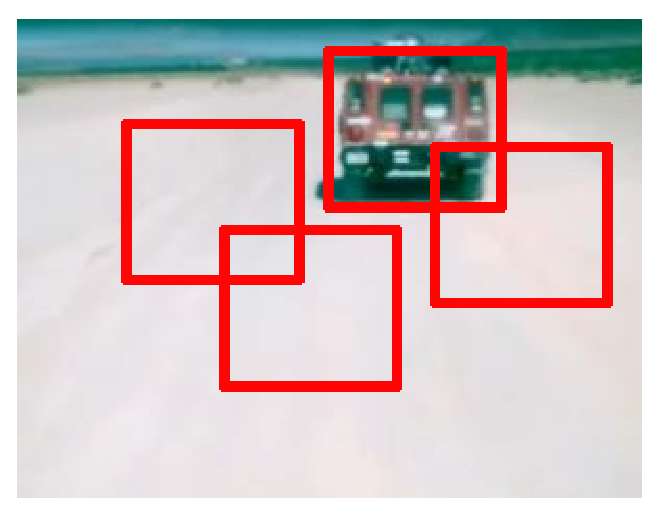
\includegraphics[width=.5\columnwidth]{images/figure2a.eps}}
  \subfloat[]{\label{subfig:(b)} 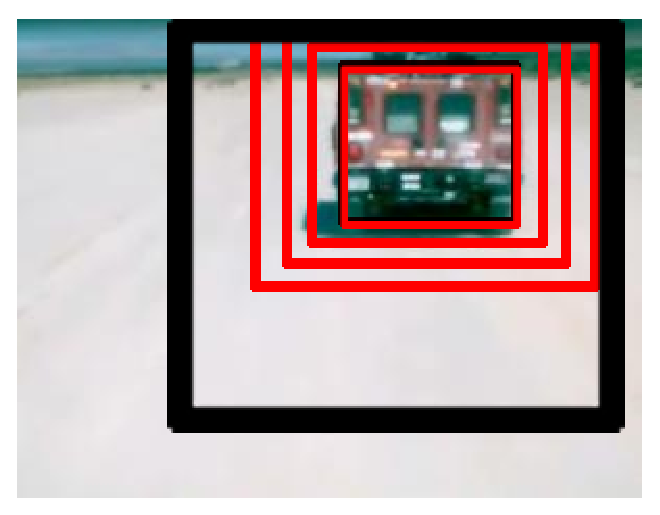
\includegraphics[width=.5\columnwidth]{images/figure2b.eps}}
  \caption{The red boxes show the analyzed regions and the black boxes represent the $WOS$. 
  (a) The regions are compared with a $ROI$ using the same scale. 
  (b) The regions are compared with a $ROI$ using different scales.}
  \label{fig:multires}
\end{figure}

The Algorithm \ref{alg:multires} describe the method explicated in the 
Fig. \ref{fig:multires}(b), It is represented by the function 
$multiscale\_match\_criterion()$ and It is used in the Algorithm \ref{alg:system}.

\begin{algorithm}[H]
 \KwData{A $ROI$, your position $P_0$ and an image frame $I_i$. }
 \KwResult{The best matched analysis region, $AR$, your position 
 $P_{max}$ and the correlation value,$r_{max}$, with the $ROI$. }
 ~\\
 $W$: Width of $ROI$\;
 $H$: Height of $ROI$\;
 $L$: Search arm in pixels (defined by the user);
 $\alpha \leftarrow 0.8$\;
 $r_{max} \leftarrow -1.0$\;
 ~\\
    \While{$0.8 \leq \alpha \leq 1.4 $}{
      
      $A \leftarrow get\_corr\_matrix(ROI,P_0,\alpha,L,I_i)$\;

      $p_i$: position $(x_i,y_i)$ of maximum value in $A$\;

      $r \leftarrow A(p_i)$\;

      \If{$r > r_{max}$}{
	$r_{max} \leftarrow r$\;
	$P_{max} \leftarrow P_0 +p_i-(L,L)$\;
	$\alpha_{max} \leftarrow \alpha$\;
      }
      ~\\
      $\alpha \leftarrow \alpha +0.05$\;
    }
    
$AR$: Region in $I_i$, at point $P_{max}$, with size $\alpha W$ by $\alpha H$\;      
\Return $\{AR,P_{max},r_{max}\}$\;
~\\
\caption{$multiscale\_match\_criterion(ROI,P_0,I_i)$ function.}
\label{alg:multires}
\end{algorithm}
We can see that the Algorithm \ref{alg:multires} use internally
the function $get\_corr\_matrix()$, this function returns a matrix 
with the correlation values of $ROI$ with the analysis regions
inside the search window around the central point $P_0$. 
All the procedure can be seen detailed in the Algorithm \ref{alg:multires2}.

\begin{algorithm}[H]
 \KwData{A $ROI$, your position $P_0$, a departure factor $\alpha$, the search arm 
 $L$ and an image frame $I_i$. }
 \KwResult{The correlation matrix $A$, compound around the point $P_0$ of $I_i$. }
 ~\\
 $W$: Width of $ROI$\;
 $H$: Height of $ROI$\;
 $lin_0$: The first term of $P_0$\;
 $col_0$: The second term of $P_0$\;
 $A$: Creates a square matrix of $2L+1$ pixels by side and fill it with zeros\;

 ~\\
    \For{$-L \leq lin \leq L$}{
    \For{$-L \leq col \leq L$}{
      $AR$: Region in $I_i$, at point $(lin_0+lin,col_0+col)$, with size $\alpha W$ by $\alpha H$\;
      $AR \leftarrow $ rescale $AR$ to $ROI$ size\;
      
      $Q$ is filled according the Eq. (\ref{eq:Q})\;
      $A(L+lin,L+col) \leftarrow PCC(Q\times ROI,Q\times AR)$\;

    }
    }
    
\Return $A$\;
~\\
\caption{$get\_corr\_matrix(ROI,P_0,\alpha,L,I_i)$ function.}
\label{alg:multires2}
\end{algorithm}


%onde estava, onde esta agora
%que tamanho tinha que tamanho tem.